\documentclass[11pt]{article}
\usepackage[utf8]{inputenc}
\usepackage[T1]{fontenc}
\usepackage[a4paper,margin=2.5cm]{geometry}
\usepackage{amsmath,amssymb}
\usepackage{booktabs}
\usepackage{graphicx}
\usepackage{xcolor}
\usepackage{natbib}
\usepackage[colorlinks=true,linkcolor=blue,citecolor=blue,urlcolor=blue]{hyperref}

\newcommand{\PR}{\mathbb{P}}
\newcommand{\given}{\,\vert\,}
\newcommand{\LR}{\mathrm{LR}}
\newcommand{\odds}{\mathrm{odds}}

\title{\textbf{Conditional Credit Pricing as Bayesian Default Updating:\\
The Correlated-Signal Problem}}
\author{Paolo Mastrogiacomo}
\date{June 2026}

\begin{document}
\maketitle

\begin{abstract}
A credit spread encodes a prior probability of default; news about an issuer is
evidence; the fair default probability is the Bayesian posterior. We make this
correspondence explicit and operational, mapping spreads to priors through the
credit triangle and revising them with likelihood ratios estimated from history.
We then isolate the failure mode that an na\"ive implementation invites: because
credit signals such as a downgrade and an earnings miss are typically driven by a
common deterioration, multiplying their likelihood ratios as if they were
independent overstates default risk. On a synthetic issuer panel the product of
marginal likelihood ratios is $8.5$ where the joint ratio is only $3.5$, and a
name carrying all three signals receives a na\"ive posterior of $14.8\%$ against a
correlation-aware $6.7\%$. A single population-wide joint ratio is not a remedy
either: with credit rating as a confounder it understates. A hierarchical Bayesian
logistic model that conditions on rating and treats the signals jointly is the best
calibrated out of sample (Brier $0.0575$ versus $0.0591$ na\"ive and $0.0657$
prior-only). The exercise reframes a standard probability puzzle as the daily
mechanics of a credit relative-value desk.
\end{abstract}

\section{Introduction}
The classic medical-test puzzle---a positive result on a rare condition leaves the
patient probably healthy---and the pricing of an issuer's default risk are the same
object \citep{gigerenzer1995}. Both begin with a base rate, observe evidence, and
update. In credit the base rate is not invented: it is quoted by the market through
the spread. Under a reduced-form view \citep{jarrowturnbull1995,duffiesingleton1999}
the spread implies a default intensity, hence a prior default probability. Each
subsequent piece of news---a rating downgrade, an earnings miss, a spread move---is
evidence with a likelihood ratio, and Bayes' rule in odds form prescribes exactly
how the implied default probability should move. If the market price has not moved
as much as the likelihood ratios imply, there may be a trade.

This paper sets out that correspondence and then studies the complication that makes
it nontrivial in practice. Real credit signals are not conditionally independent:
the same underlying deterioration tends to trigger several of them at once. Treating
them as independent confirmations---multiplying likelihood ratios---double-counts the
shared information and produces overconfident default probabilities. We quantify the
effect and show that the natural fix must account both for the correlation among
signals and for rating heterogeneity, which a hierarchical Bayesian model does.

\section{The framework}
\paragraph{Prior from the spread.}
For a constant default intensity $\lambda$ and recovery $R$, the credit triangle gives
$\lambda = s/(1-R)$ for a spread $s$, a survival probability $S(T)=e^{-\lambda T}$,
and a prior default probability
\begin{equation}
\pi \;=\; \PR(\text{default})\;=\;1-e^{-\lambda T}
       \;=\;1-\exp\!\Big(-\tfrac{s}{1-R}\,T\Big).
\end{equation}
For $R=0.4$ and $T=1$, a $121$\,bp spread implies $\pi\approx 2.0\%$.

\paragraph{Evidence and likelihood ratios.}
For a binary signal $E$ and default indicator $D$, the likelihood ratio is
$\LR(E)=\PR(E\given D)/\PR(E\given \lnot D)$, estimated from historical frequencies
with Laplace smoothing.

\paragraph{Updating in odds form.}
With prior odds $\pi/(1-\pi)$ and conditionally independent signals $E_1,\dots,E_k$,
\begin{equation}\label{eq:odds}
\underbrace{\frac{\PR(D\given E_{1:k})}{\PR(\lnot D\given E_{1:k})}}_{\text{posterior odds}}
=\underbrace{\frac{\pi}{1-\pi}}_{\text{prior odds}}\;\prod_{j=1}^{k}\LR(E_j),
\qquad
\PR(D\given E_{1:k})=\frac{\odds}{1+\odds}.
\end{equation}
Equation~\eqref{eq:odds} is the engine: prior from the spread, multiplied by the
likelihood ratio of each new signal.

\section{The independence trap}
The product in \eqref{eq:odds} is exact only when the signals are conditionally
independent given $D$. Credit signals violate this. Writing the correlation-aware
\emph{joint} likelihood ratio
$\LR(E_1\cap\dots\cap E_k)=\PR(E_1\cap\dots\cap E_k\given D)/
\PR(E_1\cap\dots\cap E_k\given \lnot D)$,
positive dependence makes
$\prod_j \LR(E_j) > \LR(E_1\cap\dots\cap E_k)$, so the na\"ive update overstates the
posterior. Table~\ref{tab:lr} shows the gap on the synthetic panel of
Section~\ref{sec:exp}: three signals with marginal ratios near $2$ multiply to $8.5$,
while their joint ratio is only $3.5$. Starting from a $2\%$ prior, a name carrying
all three is assigned $14.8\%$ na\"ively but $6.7\%$ once the redundancy is removed.

\begin{table}[h]
\centering
\begin{tabular}{lc}
\toprule
Quantity & Value \\
\midrule
$\LR(\text{downgrade})$        & 2.12 \\
$\LR(\text{earnings miss})$    & 1.96 \\
$\LR(\text{spread widening})$  & 2.04 \\
Product of marginals           & 8.50 \\
Joint $\LR$ (all three)        & 3.54 \\
\midrule
Na\"ive posterior PD (2\% prior)        & 14.8\% \\
Correlation-aware posterior PD          & \phantom{0}6.7\% \\
\bottomrule
\end{tabular}
\caption{Marginal likelihood ratios multiply far above the joint ratio, so the
independence assumption inflates the posterior.}
\label{tab:lr}
\end{table}

\section{A hierarchical Bayesian model}
A single population-wide joint ratio is not a sufficient remedy, because credit
rating confounds the relationship: pooling across ratings makes the joint ratio
understate risk for any given rating. We therefore model the default outcome of
issuer $i$ with a hierarchical logistic specification,
\begin{equation}
\mathrm{logit}\,p_i = a_{r(i)} + \sum_{k}\beta_k\,x_{ik},\quad
a_r \sim \mathcal{N}(\mu_a,\sigma_a),\quad
\beta_k \sim \mathcal{N}(0,1.5),\quad
D_i \sim \mathrm{Bernoulli}(p_i),
\end{equation}
with partial pooling of the rating intercepts $a_r$ and signals $x_{ik}$ entered
jointly, so each $\exp(\beta_k)$ is a rating- and co-signal-adjusted odds multiplier.
Inference is by NUTS in PyMC \citep{pymc2023,gelman2013}.

\section{Synthetic experiments}\label{sec:exp}
Each issuer draws a rating, a latent deterioration $z\sim\mathcal{N}(0,1)$, and a
default outcome with $\mathrm{logit}\,p = a_{r} + \gamma z$. The three signals load
on the same $z$, inducing the cross-signal correlation that defeats independence,
while the observed spread is generated from the rating-implied prior plus noise (a
deliberately stale prior, so the signals carry new information). We fit on $60\%$ of
$6{,}000$ issuers and evaluate on the rest.

\section{Results}
Table~\ref{tab:bt} reports holdout performance for three predictors: the spread
prior alone, the na\"ive independent update, and the Bayesian posterior. Updating on
signals helps (AUC $0.767\to0.837$); accounting for their correlation and for rating
heterogeneity helps further and improves calibration (Brier $0.0591\to0.0575$, log
loss $0.2100\to0.2056$). Figure~\ref{fig:cal} shows the na\"ive curve bowing above
the diagonal in the high-probability region---overstated risk---while the Bayesian
curve tracks the diagonal. On names carrying two or more signals the na\"ive
predictor runs hotter than the correlation-aware model ($17.4\%$ versus $13.9\%$),
the redundancy bias made concrete.

\begin{table}[h]
\centering
\begin{tabular}{lccc}
\toprule
Predictor & AUC & Brier & Log loss \\
\midrule
Prior-only (spread)        & 0.767 & 0.0657 & 0.2458 \\
Na\"ive independent $\LR$  & 0.837 & 0.0591 & 0.2100 \\
Hierarchical Bayesian      & \textbf{0.842} & \textbf{0.0575} & \textbf{0.2056} \\
\bottomrule
\end{tabular}
\caption{Out-of-sample performance ($n=2{,}400$ holdout issuers).}
\label{tab:bt}
\end{table}

\begin{figure}[h]
\centering
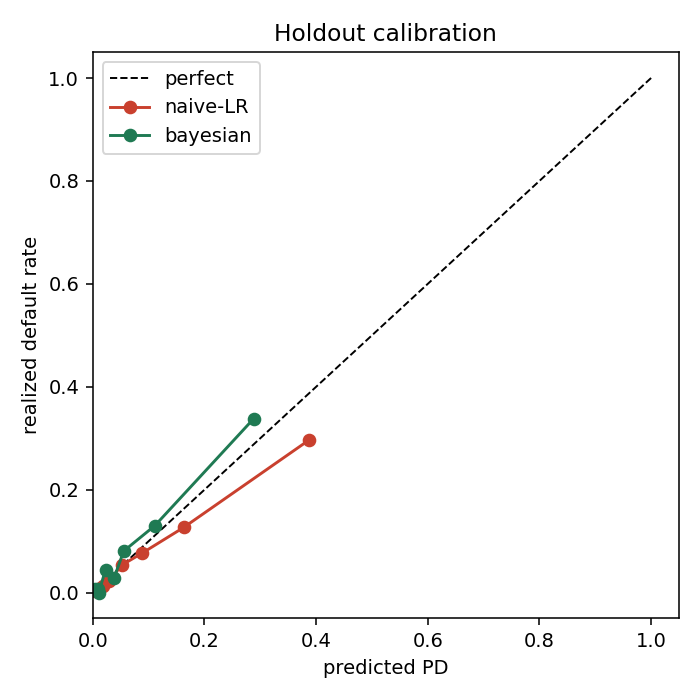
\includegraphics[width=0.46\textwidth]{figures/calibration.png}
\caption{Holdout calibration. The na\"ive update (red) overstates default
probability for high-risk names; the hierarchical Bayesian model (green) is closer
to the diagonal.}
\label{fig:cal}
\end{figure}

\section{Discussion}
The contribution is conceptual as much as empirical: the spread-implied prior times
likelihood-ratio update is the mechanics of conditional credit pricing, and it is
the same operation as the textbook test-positive puzzle. The practical caution is
that signals are correlated, so the independence shortcut produces overconfident
default probabilities; the appropriate correction conditions jointly on the signals
and on rating. Limitations are clear: the data are synthetic, the signals binary and
static, and the model omits the term structure of hazards. Natural extensions are
real rating-migration and CDS data, continuous and time-stamped signals, a
copula treatment of the joint likelihood, and a mapping from posterior default
probabilities back to fair spreads to define explicit relative-value signals.

\bibliographystyle{plainnat}
\bibliography{references}
\end{document}
